% Fig 1 — SensingPolarPredictor architecture (EDITABLE TikZ SKELETON, not final art).
% Matches the ACTUAL forward graph in src/models/sensing_polar.py :: SensingPolarPredictor.forward
% (Checklist D): radar/lidar encoders -> cross-attention fusion -> 3 branches (radar/lidar/fused)
% x 2 heads (angle B_theta=64, range B_r=8) -> confidence_combine -> top-K shortlist -> RF verify.
% RADAR path drawn as the visual PRIMARY SPINE (radar-primary paper, D-015); fusion present, not
% oversold. Compile standalone:  pdflatex fig1_architecture.tex
\documentclass[border=4pt]{standalone}
\usepackage{times}                 % Times-equivalent serif to match ieee_style.mplstyle
\usepackage{amsmath}
\usepackage{tikz}
\usetikzlibrary{positioning, arrows.meta, fit, backgrounds, calc}

\begin{document}
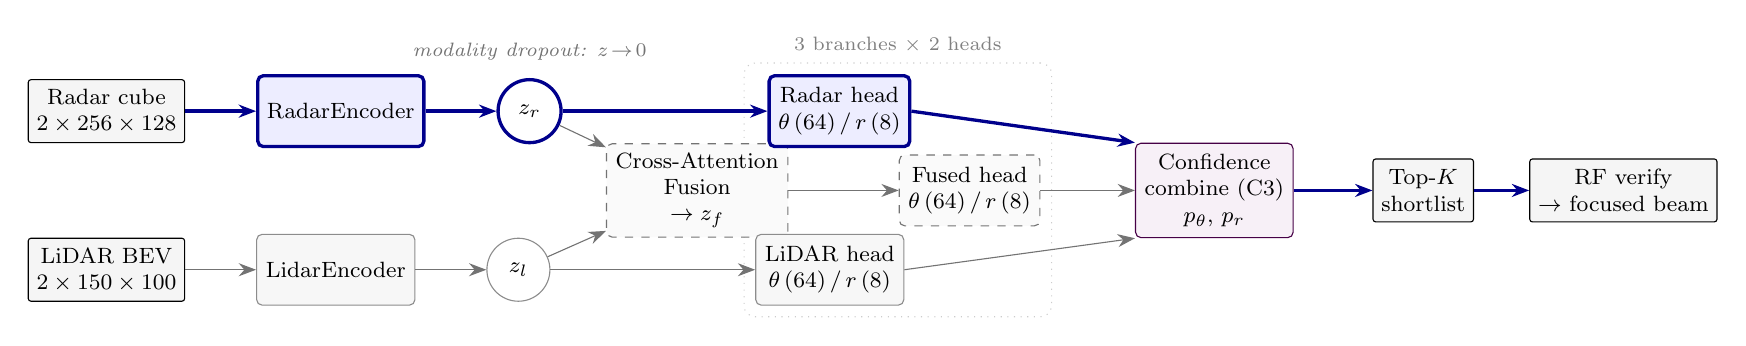
\begin{tikzpicture}[
  font=\footnotesize,
  >={Stealth[length=2.2mm]},
  io/.style    ={draw, rounded corners=1pt, fill=black!4,  minimum height=8mm, align=center, inner sep=3pt},
  enc/.style   ={draw, rounded corners=2pt, minimum height=9mm, minimum width=16mm, align=center},
  prim/.style  ={enc, very thick, draw=blue!55!black, fill=blue!7},      % radar = primary spine
  sec/.style   ={enc, draw=black!45, fill=black!3},                      % lidar = secondary
  fuse/.style  ={draw, rounded corners=2pt, dashed, draw=black!55, fill=black!2, align=center, minimum height=9mm},
  head/.style  ={draw, rounded corners=2pt, minimum height=11mm, minimum width=15mm, align=center},
  comb/.style  ={draw, rounded corners=2pt, fill=violet!6, draw=violet!55!black, align=center, minimum height=12mm},
  pflow/.style ={->, very thick, blue!55!black},                        % primary (radar) data flow
  flow/.style  ={->, black!55},                                         % secondary / shared flow
]

% ---- column 1: inputs ----
\node[io] (radin) {Radar cube\\$2\times256\times128$};
\node[io, below=12mm of radin] (lidin) {LiDAR BEV\\$2\times150\times100$};

% ---- column 2: encoders ----
\node[prim, right=9mm of radin] (renc) {RadarEncoder};
\node[sec,  right=9mm of lidin] (lenc) {LidarEncoder};

% ---- column 3: latents + fusion ----
\node[draw, circle, right=9mm of renc, minimum size=8mm, very thick, draw=blue!55!black] (zr) {$z_r$};
\node[draw, circle, right=9mm of lenc, minimum size=8mm, draw=black!45] (zl) {$z_l$};
\node[fuse] (fus) at ($(zr)!0.5!(zl) + (22mm,0)$) {Cross-Attention\\Fusion\\$\rightarrow z_f$};

% ---- column 4: three branch heads (each PolarHead: angle 64 + range 8) ----
\node[head, prim, right=26mm of zr] (hr) {Radar head\\$\theta$\,(64)\,/\,$r$\,(8)};
\node[head, fuse, right=14mm of fus] (hf) {Fused head\\$\theta$\,(64)\,/\,$r$\,(8)};
\node[head, sec,  right=26mm of zl] (hl) {LiDAR head\\$\theta$\,(64)\,/\,$r$\,(8)};

% ---- column 5: confidence-weighted combine ----
\node[comb, right=12mm of hf] (cc) {Confidence\\combine (C3)\\$p_\theta,\,p_r$};

% ---- column 6: shortlist + RF verification ----
\node[io, right=10mm of cc] (topk) {Top-$K$\\shortlist};
\node[io, right=7mm of topk] (rf) {RF verify\\$\rightarrow$ focused beam};

% ---- flows: radar = primary spine (thick blue) ----
\draw[pflow] (radin) -- (renc);
\draw[pflow] (renc)  -- (zr);
\draw[pflow] (zr)    -- (hr);
\draw[pflow] (hr.east) -- (cc.north west);

% ---- flows: lidar = secondary ----
\draw[flow] (lidin) -- (lenc);
\draw[flow] (lenc)  -- (zl);
\draw[flow] (zl)    -- (hl);
\draw[flow] (hl.east) -- (cc.south west);

% ---- flows: into fusion (both latents) and fused head ----
\draw[flow] (zr) -- (fus);
\draw[flow] (zl) -- (fus);
\draw[flow] (fus) -- (hf);
\draw[flow] (hf) -- (cc);

% ---- flows: combine -> top-K -> RF verify ----
\draw[pflow] (cc)   -- (topk);
\draw[pflow] (topk) -- (rf);

% ---- modality-dropout annotation (z zeroed at train aug / missing-sensor eval) ----
\node[font=\scriptsize\itshape, text=black!55, above=1mm of zr] {modality dropout: $z\!\to\!0$};

% ---- group label: 3 branches ----
\begin{scope}[on background layer]
  \node[draw=black!20, dotted, rounded corners, fit=(hr)(hf)(hl),
        inner sep=4pt, label={[font=\scriptsize, text=black!50]above:3 branches $\times$ 2 heads}] {};
\end{scope}

\end{tikzpicture}
\end{document}
